\documentclass{beamer}
\mode<presentation>
\usetheme{CambridgeUS}
\usepackage[russian]{babel}
\usepackage[utf8]{inputenc}
\usepackage[T2A]{fontenc}
\usepackage{sansmathaccent}

\usepackage{verbatim}
\usepackage{alltt}

\pdfmapfile{+sansmathaccent.map}
\title[СУБД]{Структуры базы данных. Нормализация}
\author{Наумов Д.А., доц. каф. КТ}
\date[22.03.2019] {Основы компьютерных наук (3 часть), 2019}

\begin{document}

%ТИТУЛЬНЫЙ СЛАЙД
\begin{frame}
  \titlepage
\end{frame}
  
%СОДЕРЖАНИЕ ЛЕКЦИИ
\begin{frame}
  \frametitle{Содержание лекции}
  \tableofcontents  
\end{frame}
  
%РАЗДЕЛ 1
\section{Нормализация}
\begin{frame}
\begin{itemize}
\item Нормализация схемы реляционной БД оказывает существенное влияние буквально на все аспекты взаимодействия с БД: от затрат на модификацию структур и данных до производительности запросов приложений и хранимых объёмов информации. 
\item В ряде случаев структуры могут быть сознательно  денормализованы.
\item Нормализация — не догма, но чтобы её нарушать, нужны основания
\item На практике проектирования схем баз данных достижение третьей нормальной формы (3НФ) считается достаточным условием для большинства случаев.
\end{itemize}
\end{frame} 

\begin{frame}
\begin{block}{Основные свойства нормальных форм}
\begin{itemize}
\item каждая следующая нормальная форма в некотором смысле улучшает свойства предыдущей;
\item при переходе к следующей нормальной форме свойства предыдущих нормальных форм сохраняются;
\end{itemize}
\end{block}

\begin{center}
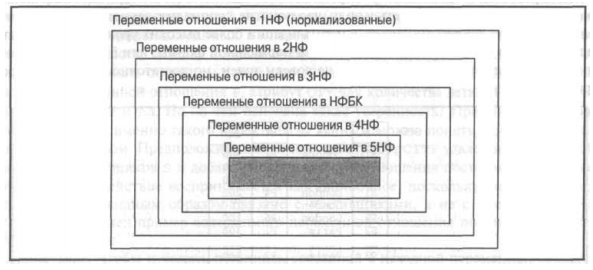
\includegraphics[scale=0.4]{images/forms.png}
\end{center}

\begin{block}{Схемы БД называются эквивалентными}
если содержание исходной БД может быть получено путем эквивалентного соединения отношений, входящих в результирующую схему, и при этом не появляется новых кортежей.
\end{block}
\end{frame} 

\begin{frame}
\begin{block}{1НФ - первая нормальная форма}
выполняется, если все значения атрибутов (колонок таблицы) атомарны, то есть неделимы.
\end{block}
\begin{itemize}
\item cобственные типы данных СУБД считаются атомарными, исключение
могут составлять массивы, в том числе символьные (текстовые) и байтовые.
\item атомарность может быть относительна выбранного взгляда со стороны предметной области и контекста. \end{itemize}
Пример 1: телефонный номер (в базе данных маркетинга, у телефонных операторов), колонки для хранения комментариев, целая и дробная части действительного числа, дата-время.

Пример 2: фамилия, имя, отчество в одной колонке.
\end{frame} 

\begin{frame}
\begin{block}{Пример}
\begin{center}
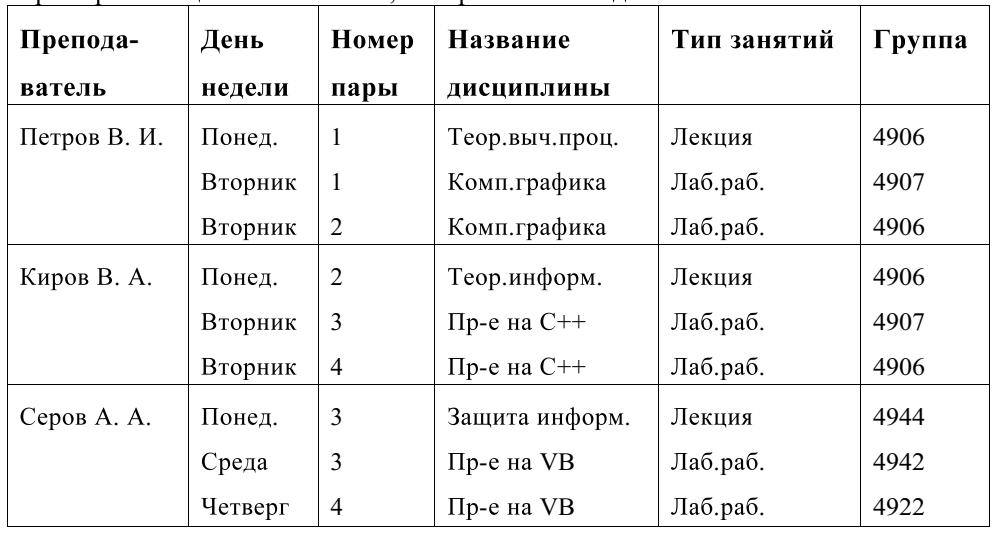
\includegraphics[scale=0.4]{images/nf-0.png}
\end{center}
\end{block}
\end{frame}

\begin{frame}
\begin{block}{Пример}
\begin{center}
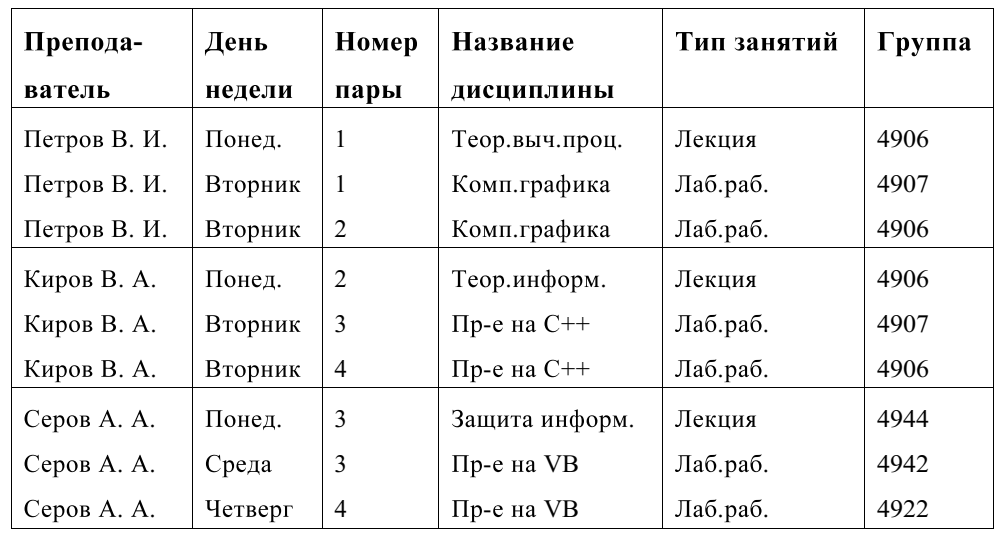
\includegraphics[scale=0.4]{images/nf-1.png}
\end{center}
\end{block}
\end{frame}

\begin{frame}
\begin{block}{2НФ - вторая нормальная форма}
означает, что выполнены требования 1НФ, при этом все атрибуты целиком зависят от составного ключа и не
зависят ни от какой его части.
\end{block}
\begin{itemize}
\item в определении говорится о ключах вообще, а не только о первичных. 
\item в отношении может быть несколько ключей, и некоторые из них могут являться составными
\end{itemize}
Пример 1: Описание продаж товара.

Пример 2: Сдача сессии (ФИО, №Зачетки, Группа, Дисциплина, Оценка).

Пример 3: Ключ - атрибут не выделенной еще сущности.
\end{frame}

\begin{frame}
\begin{block}{3НФ - вторая нормальная форма}
означает, что выполнены требования 2НФ, при этом в между атрибутами отношения нет транзитивных
зависимостей.
\end{block}
Пример: продажа каждой товарной позиции имеет своим основанием документ (заказ, счёт и т.д.), а её стоимость характеризуется ценой, количеством и валютой.

Транзитивные зависимости:
\begin{itemize}
\item Идентификатор продажи $\rightarrow$ Номер документа
\item Идентификатор продажи $\rightarrow$ Код валюты
\item Номер документа $\rightarrow$ Код валюты
\end{itemize}
Результатом нарушения 3НФ является избыточность хранения и необходимость обновления данных в связанной таблице.
\end{frame}

\begin{frame}
Пример: (ФИО, Номер зачетки, Группа, Факультет, Специальность, Выпускающая кафедра)
\begin{block}{Пример}
\begin{center}
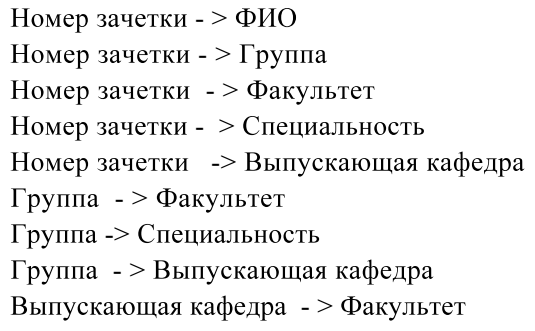
\includegraphics[scale=0.5]{images/nf-3.png}
\end{center}
\end{block}
\end{frame}

\section{Типы приложений: транзакционная и аналитическая обработка}
\begin{frame}
OLTP (On-Line Transaction Processing) — интерактивная транзакционная обработка.
\begin{itemize}
\item Обработка идёт в режиме реального или приближенного к реальному времени.
\item Запросы представляют собой интенсивный поток коротких операций по вставке, изменению и удалению небольшого числа записей в БД.
\end{itemize}
OLAP (On-Line Analytical Processing) - интерактивная аналитическая обработка. 
\begin{itemize}
\item Данные находятся \textbf{в режиме чтения}, за исключением моментов их обновления.
\item Выборки представляют собой \textbf{одиночные тяжёлые запросы}: поиски и расчёты по множеству произвольных критериев.
\item \textbf{Время отклика системы не регламентировано}.
\item Размеры базы данных на порядок и больше транзакционных.
\end{itemize}
\end{frame}

\section{Денормализация}
\begin{frame}
Цели нормализации:
\begin{itemize}
\item устранение избыточности при хранении данных, приводящей к увеличению размера БД.
\item исключение необходимости модификации данных в связных таблицах для минимизации времени и операций, проводящихся в одной транзакции.
\end{itemize}
В приложениях интерактивной аналитической обработки приоритет меняется: на первый план выходит время отклика системы, в ущерб которому данные могут быть избыточны.
\end{frame}

\begin{frame}
Допустимые схемы для OLAP: "снежинка", "звезда":
\begin{itemize}
\item центральным элементом являются таблицы фактов, содержащие события, транзакции, документы и др.
\item в таблице фактов одному документу (каждой его строке), соответствует одна запись.
\end{itemize}
\begin{block}{Денормализация документов в таблицу фактов}
\begin{center}
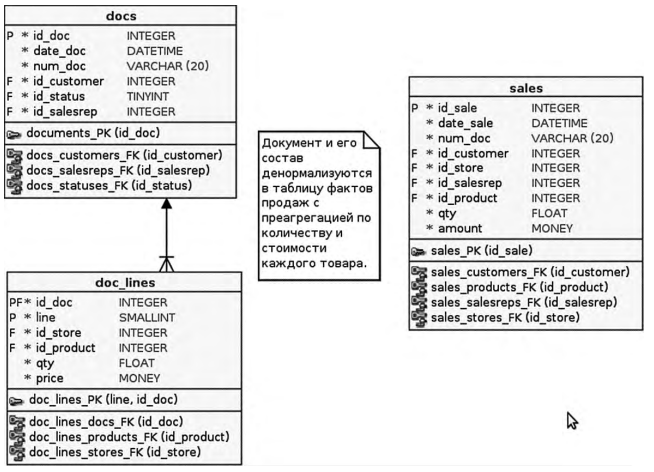
\includegraphics[scale=0.4]{images/denorm.png}
\end{center}
\end{block}
\end{frame}

\begin{frame}
\begin{block}{Пример SQL-запроса в транзакционной СУБД}
\begin{center}
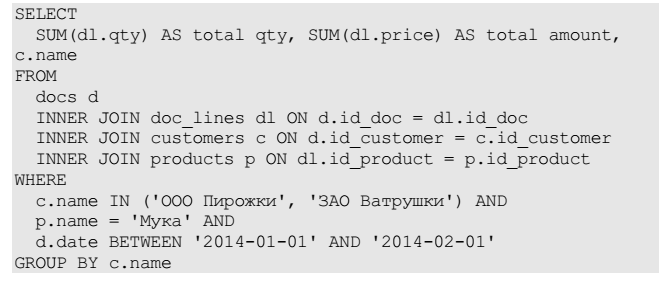
\includegraphics[scale=0.45]{images/sql-trans.png}
\end{center}
\end{block}
\begin{block}{Пример SQL-запроса в OLAP-СУБД}
\begin{center}
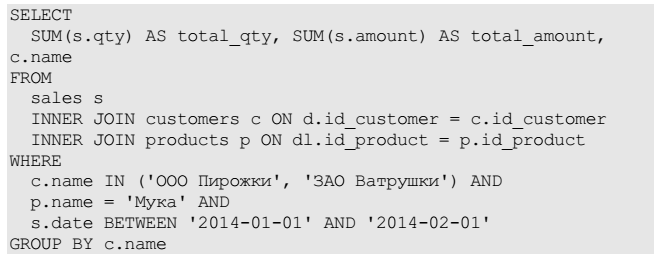
\includegraphics[scale=0.45]{images/sql-analitic.png}
\end{center}
\end{block}
\end{frame}

\begin{frame}
Если таблица фактов ссылается на таблицы-измерения, имеющие ссылки на другие измерения, то такая схема называется "снежинка".
\begin{block}{Таблица фактов в схеме "снежинка"}
\begin{center}
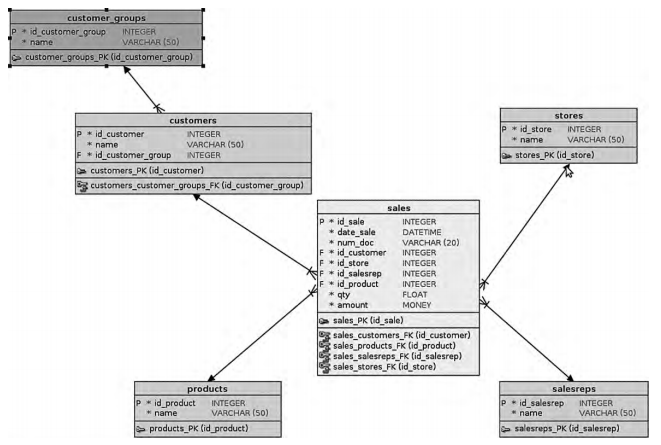
\includegraphics[scale=0.45]{images/snow.png}
\end{center}
\end{block}
Для запросов, включающих фильтрацию по группам клиентов, приходится делать дополнительное соединение.
\end{frame}

\begin{frame}
Схема "Звезда" полностью исключает иерархию измерений и необходимость соединения соответствующих таблиц в одном запросе.
\begin{block}{Таблица фактов в схеме "звезда"}
\begin{center}
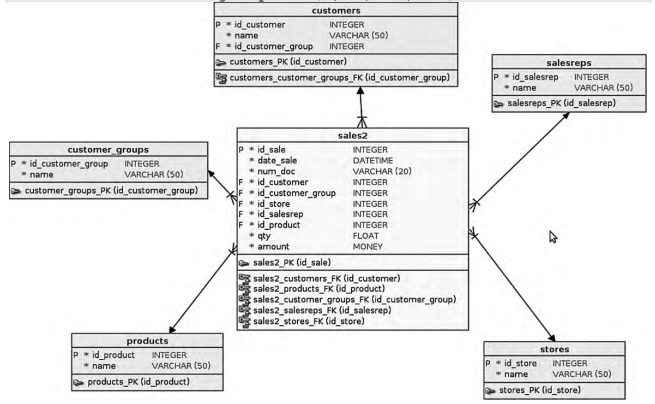
\includegraphics[scale=0.45]{images/star.png}
\end{center}
\end{block}
Обратной стороной денормализации всегда является избыточность, являющаяся причиной увеличения размера БД как в случае транзакционных, так и аналитических приложений.
\end{frame}


\begin{frame}
\begin{block}{Пример SQL-запроса в схеме "снежинка"}
\begin{center}
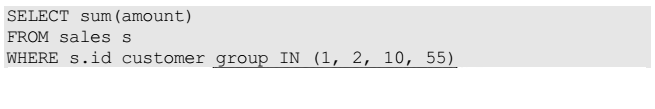
\includegraphics[scale=0.5]{images/star-sql.png}
\end{center}
\end{block}
\begin{block}{Пример SQL-запроса в схеме "звезда"}
\begin{center}
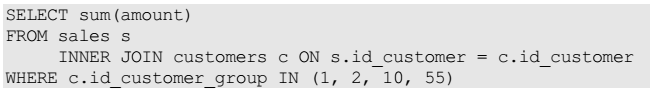
\includegraphics[scale=0.5]{images/snow-sql.png}
\end{center}
\end{block}
\begin{block}{Задача}
Посчитаем, примерную дельту на приведённом выше примере преобразования
"снежинки" в "звезду", если таблица продаж не использует компрессию данных и содержит
около 500 миллионов строк, а количество групп покупателей порядка 1000.
\end{block}
\end{frame}

\begin{frame}
\begin{block}{Пример типовой архитектуры OLAP}
\begin{center}
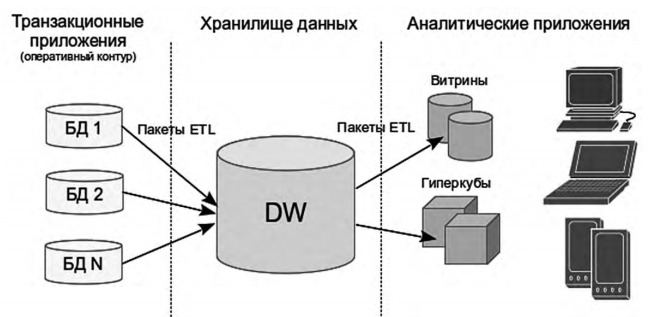
\includegraphics[scale=0.5]{images/olap.png}
\end{center}
\end{block}
\begin{itemize}
\item тяжёлые запросы по произвольным критериям выборки.
\item разделение собственно хранилища (data warehouse), где данные представлены в
минимально агрегированном виде, и конечных БД, адаптированных под
нужды пользователей разных профилей и предметных областей.
\end{itemize}
\end{frame}

\begin{frame}
\begin{block}{Пример типовой архитектуры OLAP}
\begin{center}
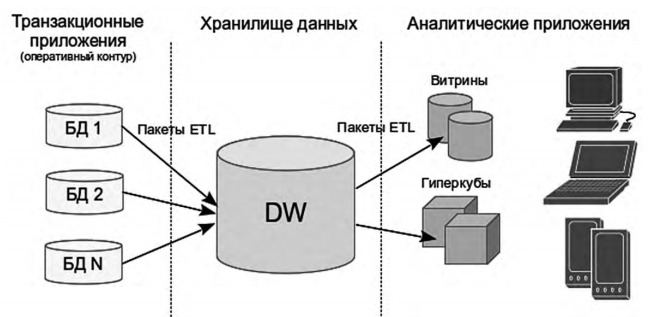
\includegraphics[scale=0.5]{images/olap.png}
\end{center}
\end{block}
\begin{itemize}
\item в роли баз данных конечных пользователей могут выступать как вполне
реляционные витрины данных (datamart), так и другие типы СУБД, прежде
всего, основанные на многомерных моделях.
\item витрина данных представляет собой реляционную БД или даже одну
таблицу фактов, содержащую более агрегированную и отфильтрованную
информацию, извлечённую непосредственно из хранилища данных.
\end{itemize}
\end{frame}

\end{document}